
%\documentclass[11pts,a4paper,amsmath,amssymb,floatfix]{article}%{report}%{book}
\documentclass[12pts,a4paper,amsmath,amssymb,floatfix]{article}%{report}%{book}
\usepackage{graphicx,wrapfig,pdfpages}% Include figure files
%\usepackage{dcolumn,enumerate}% Align table columns on decimal point
\usepackage{enumerate,enumitem}% Align table columns on decimal point
\usepackage{bm,dpfloat}% bold math
\usepackage[pdftex,bookmarks,colorlinks=true,urlcolor=rltblue,citecolor=blue]{hyperref}
\usepackage{amsfonts,amsmath,amssymb,stmaryrd,indentfirst}
\usepackage{times,psfrag}
\usepackage{natbib}
\usepackage{color}
\usepackage{units}
\usepackage{rotating}
\usepackage{multirow}


\usepackage{pifont}
\usepackage{subfigure}
\usepackage{subeqnarray}
\usepackage{ifthen}

\usepackage{supertabular}
\usepackage{moreverb}
\usepackage{listings}
\usepackage{palatino}
%\usepackage{doi}
\usepackage{longtable}
\usepackage{float}
\usepackage{perpage}
\MakeSorted{figure}
%\usepackage{pdflscape}


%\usepackage{booktabs}
%\newcommand{\ra}[1]{\renewcommand{\arraystretch}{#1}}


\definecolor{rltblue}{rgb}{0,0,0.75}


%\usepackage{natbib}
\usepackage{fancyhdr} %%%%
\pagestyle{fancy}%%%%
% with this we ensure that the chapter and section
% headings are in lowercase
%%%%\renewcommand{\chaptermark}[1]{\markboth{#1}{}}
\renewcommand{\sectionmark}[1]{\markright{\thesection\ #1}}
\fancyhf{} %delete the current section for header and footer
\fancyhead[LE,RO]{\bfseries\thepage}
\fancyhead[LO]{\bfseries\rightmark}
\fancyhead[RE]{\bfseries\leftmark}
\renewcommand{\headrulewidth}{0.5pt}
% make space for the rule
\fancypagestyle{plain}{%
\fancyhead{} %get rid of the headers on plain pages
\renewcommand{\headrulewidth}{0pt} % and the line
}

\def\newblock{\hskip .11em plus .33em minus .07em}
\usepackage{color}

%\usepackage{makeidx}
%\makeindex

\setlength\textwidth      {16.cm}
\setlength\textheight     {22.6cm}
\setlength\oddsidemargin  {-0.3cm}
\setlength\evensidemargin {0.3cm}

\setlength\headheight{14.49998pt} 
\setlength\topmargin{0.0cm}
\setlength\headsep{1.cm}
\setlength\footskip{1.cm}
\setlength\parskip{0pt}
\setlength\parindent{0pt}


%%%
%%% Headers and Footers
\lhead[] {\text{\small{EX3029 -- Chemical Thermodynamics}}} 
\rhead[] {{\text{\small{Extra-Examples - Module 06}}}}
%\chead[] {\text{\small{Session 2012/13}}} 
\lfoot[]{Dr Jeff Gomes}
%\cfoot[\thepage]{\thepage}
\rfoot[\text{\small{\thepage}}]{\thepage}
\renewcommand{\headrulewidth}{0.8pt}


%%%
%%% space between lines
%%%
\renewcommand{\baselinestretch}{1.5}

\newenvironment{VarDescription}[1]%
  {\begin{list}{}{\renewcommand{\makelabel}[1]{\textbf{##1:}\hfil}%
    \settowidth{\labelwidth}{\textbf{#1:}}%
    \setlength{\leftmargin}{\labelwidth}\addtolength{\leftmargin}{\labelsep}}}%
  {\end{list}}

%%%%%%%%%%%%%%%%%%%%%%%%%%%%%%%%%%%%%%%%%%%
%%%%%%                              %%%%%%%
%%%%%%      NOTATION SECTION        %%%%%%%
%%%%%%                              %%%%%%%
%%%%%%%%%%%%%%%%%%%%%%%%%%%%%%%%%%%%%%%%%%%

% Text abbreviations.
\newcommand{\ie}{{\em{i.e., }}}
\newcommand{\eg}{{\em{e.g., }}}
\newcommand{\cf}{{\em{cf., }}}
\newcommand{\wrt}{with respect to}
\newcommand{\lhs}{left hand side}
\newcommand{\rhs}{right hand side}
% Commands definining mathematical notation.

% This is for quantities which are physically vectors.
\renewcommand{\vec}[1]{{\mbox{\boldmath$#1$}}}
% Physical rank 2 tensors
\newcommand{\tensor}[1]{\overline{\overline{#1}}}
% This is for vectors formed of the value of a quantity at each node.
\newcommand{\dvec}[1]{\underline{#1}}
% This is for matrices in the discrete system.
\newcommand{\mat}[1]{\mathrm{#1}}


\DeclareMathOperator{\sgn}{sgn}
\newtheorem{thm}{Theorem}[section]
\newtheorem{lemma}[thm]{Lemma}

%\newcommand\qed{\hfill\mbox{$\Box$}}
\newcommand{\re}{{\mathrm{I}\hspace{-0.2em}\mathrm{R}}}
\newcommand{\inner}[2]{\langle#1,#2\rangle}
\renewcommand\leq{\leqslant}
\renewcommand\geq{\geqslant}
\renewcommand\le{\leqslant}
\renewcommand\ge{\geqslant}
\renewcommand\epsilon{\varepsilon}
\newcommand\eps{\varepsilon}
\renewcommand\phi{\varphi}
\newcommand{\bmF}{\vec{F}}
\newcommand{\bmphi}{\vec{\phi}}
\newcommand{\bmn}{\vec{n}}
\newcommand{\bmns}{{\textrm{\scriptsize{\boldmath $n$}}}}
\newcommand{\bmi}{\vec{i}}
\newcommand{\bmj}{\vec{j}}
\newcommand{\bmk}{\vec{k}}
\newcommand{\bmx}{\vec{x}}
\newcommand{\bmu}{\vec{u}}
\newcommand{\bmv}{\vec{v}}
\newcommand{\bmr}{\vec{r}}
\newcommand{\bma}{\vec{a}}
\newcommand{\bmg}{\vec{g}}
\newcommand{\bmU}{\vec{U}}
\newcommand{\bmI}{\vec{I}}
\newcommand{\bmq}{\vec{q}}
\newcommand{\bmT}{\vec{T}}
\newcommand{\bmM}{\vec{M}}
\newcommand{\bmtau}{\vec{\tau}}
\newcommand{\bmOmega}{\vec{\Omega}}
\newcommand{\pp}{\partial}
\newcommand{\kaptens}{\tensor{\kappa}}
\newcommand{\tautens}{\tensor{\tau}}
\newcommand{\sigtens}{\tensor{\sigma}}
\newcommand{\etens}{\tensor{\dot\epsilon}}
\newcommand{\ktens}{\tensor{k}}
\newcommand{\half}{{\textstyle \frac{1}{2}}}
\newcommand{\tote}{E}
\newcommand{\inte}{e}
\newcommand{\strt}{\dot\epsilon}
\newcommand{\modu}{|\bmu|}
% Derivatives
\renewcommand{\d}{\mathrm{d}}
\newcommand{\D}{\mathrm{D}}
\newcommand{\ddx}[2][x]{\frac{\d#2}{\d#1}}
\newcommand{\ddxx}[2][x]{\frac{\d^2#2}{\d#1^2}}
\newcommand{\ddt}[2][t]{\frac{\d#2}{\d#1}}
\newcommand{\ddtt}[2][t]{\frac{\d^2#2}{\d#1^2}}
\newcommand{\ppx}[2][x]{\frac{\partial#2}{\partial#1}}
\newcommand{\ppxx}[2][x]{\frac{\partial^2#2}{\partial#1^2}}
\newcommand{\ppt}[2][t]{\frac{\partial#2}{\partial#1}}
\newcommand{\pptt}[2][t]{\frac{\partial^2#2}{\partial#1^2}}
\newcommand{\DDx}[2][x]{\frac{\D#2}{\D#1}}
\newcommand{\DDxx}[2][x]{\frac{\D^2#2}{\D#1^2}}
\newcommand{\DDt}[2][t]{\frac{\D#2}{\D#1}}
\newcommand{\DDtt}[2][t]{\frac{\D^2#2}{\D#1^2}}
% Norms
\newcommand{\Ltwo}{\ensuremath{L_2} }
% Basis functions
\newcommand{\Qone}{\ensuremath{Q_1} }
\newcommand{\Qtwo}{\ensuremath{Q_2} }
\newcommand{\Qthree}{\ensuremath{Q_3} }
\newcommand{\QN}{\ensuremath{Q_N} }
\newcommand{\Pzero}{\ensuremath{P_0} }
\newcommand{\Pone}{\ensuremath{P_1} }
\newcommand{\Ptwo}{\ensuremath{P_2} }
\newcommand{\Pthree}{\ensuremath{P_3} }
\newcommand{\PN}{\ensuremath{P_N} }
\newcommand{\Poo}{\ensuremath{P_1P_1} }
\newcommand{\PoDGPt}{\ensuremath{P_{-1}P_2} }

\newcommand{\metric}{\tensor{M}}
\newcommand{\configureflag}[1]{\texttt{#1}}

% Units
\newcommand{\m}[1][]{\unit[#1]{m}}
\newcommand{\km}[1][]{\unit[#1]{km}}
\newcommand{\s}[1][]{\unit[#1]{s}}
\newcommand{\invs}[1][]{\unit[#1]{s}\ensuremath{^{-1}}}
\newcommand{\ms}[1][]{\unit[#1]{m\ensuremath{\,}s\ensuremath{^{-1}}}}
\newcommand{\mss}[1][]{\unit[#1]{m\ensuremath{\,}s\ensuremath{^{-2}}}}
\newcommand{\K}[1][]{\unit[#1]{K}}
\newcommand{\PSU}[1][]{\unit[#1]{PSU}}
\newcommand{\Pa}[1][]{\unit[#1]{Pa}}
\newcommand{\kg}[1][]{\unit[#1]{kg}}
\newcommand{\rads}[1][]{\unit[#1]{rad\ensuremath{\,}s\ensuremath{^{-1}}}}
\newcommand{\kgmm}[1][]{\unit[#1]{kg\ensuremath{\,}m\ensuremath{^{-2}}}}
\newcommand{\kgmmm}[1][]{\unit[#1]{kg\ensuremath{\,}m\ensuremath{^{-3}}}}
\newcommand{\Nmm}[1][]{\unit[#1]{N\ensuremath{\,}m\ensuremath{^{-2}}}}

% Dimensionless numbers
\newcommand{\dimensionless}[1]{\mathrm{#1}}
\renewcommand{\Re}{\dimensionless{Re}}
\newcommand{\Ro}{\dimensionless{Ro}}
\newcommand{\Fr}{\dimensionless{Fr}}
\newcommand{\Bu}{\dimensionless{Bu}}
\newcommand{\Ri}{\dimensionless{Ri}}
\renewcommand{\Pr}{\dimensionless{Pr}}
\newcommand{\Pe}{\dimensionless{Pe}}
\newcommand{\Ek}{\dimensionless{Ek}}
\newcommand{\Gr}{\dimensionless{Gr}}
\newcommand{\Ra}{\dimensionless{Ra}}
\newcommand{\Sh}{\dimensionless{Sh}}
\newcommand{\Sc}{\dimensionless{Sc}}


% Journals
\newcommand{\IJHMT}{{\it International Journal of Heat and Mass Transfer}}
\newcommand{\NED}{{\it Nuclear Engineering and Design}}
\newcommand{\ICHMT}{{\it International Communications in Heat and Mass Transfer}}
\newcommand{\NET}{{\it Nuclear Engineering and Technology}}
\newcommand{\HT}{{\it Heat Transfer}}   
\newcommand{\IJHT}{{\it International Journal for Heat Transfer}}

\newcommand{\frc}{\displaystyle\frac}
\newcommand{\red}{\textcolor{red}}
\newcommand{\blue}{\textcolor{blue}}
\newcommand{\green}{\textcolor{green}}
\newcommand{\purple}{\textcolor{purple}}
 
\newlist{ExList}{enumerate}{1}
\setlist[ExList,1]{label={\bf Example 1.} {\bf \arabic*}}

\newlist{ProbList}{enumerate}{1}
\setlist[ProbList,1]{label={\bf Problem 1.} {\bf \arabic*}}

%%%%%%%%%%%%%%%%%%%%%%%%%%%%%%%%%%%%%%%%%%%
%%%%%%                              %%%%%%%
%%%%%% END OF THE NOTATION SECTION  %%%%%%%
%%%%%%                              %%%%%%%
%%%%%%%%%%%%%%%%%%%%%%%%%%%%%%%%%%%%%%%%%%%


% Cause numbering of subsubsections. 
%\setcounter{secnumdepth}{8}
%\setcounter{tocdepth}{8}

\setcounter{secnumdepth}{4}%
\setcounter{tocdepth}{4}%


\begin{document}



\begin{enumerate}[label=\bfseries Example \arabic*]

%%%
%%% Elliot & Lira (Ex 3.4)  
%%%
\item\label{Example:1} Five moles of hydrogen, two moles of CO and 1.5 moles of CH$_{3}$OH vapour are combined in a closed system methanol synthesis reactor at 500 K and 1 MPa. Develop expressions for the mole fractions of the species in terms of the reaction coordinate. The components are known to reacto with the following stoichiometry:
  \begin{displaymath}
      2 H_{2} (g) + CO (g) \Longleftrightarrow CH_{3}OH (g).
  \end{displaymath}

\bigskip

{\large{\bf Solution:}}

   \begin{itemize}
      \item We need to develop expressions for each species in the gaseous form. In the equilibrium, the molar stoichiometric coefficient and the initial number of moles are:
         \begin{displaymath}
            \nu = \sum\limits_{i}\nu_{i}= (-2)+(-1)+(+1)= -2 \;\;\text{ and }\;\; n_{0} = \sum\limits_{i}n_{i,0}= 5 + 2 + 1.5 = 8.5,
         \end{displaymath} 
         respectively.
      \item The mole fraction of each species is given by
         \begin{displaymath}
           y_{i} = \frc{n_{i}}{n} = \frc{n_{i,0}+\nu_{i}\epsilon}{n_{0}+\nu\epsilon}.
         \end{displaymath}
         with the total number of moles in equilibrium given by $n=8.5-2\epsilon$.
         \begin{displaymath}
           y_{\text{H}_{2}} = \frc{5-2\epsilon}{8.5-2\epsilon},\;\;\; y_{\text{CO}} = \frc{2-\epsilon}{8.5-2\epsilon}\;\;\text{ and }\;\; y_{\text{CH}_{3}\text{OH}}=\frc{1.5+\epsilon}{8.5-2\epsilon}
         \end{displaymath}
   \end{itemize}
\clearpage

\begin{comment}
%%%
%%%   
%%%
\item\label{Example:2} Consider the chemical reaction,
         \begin{displaymath}
             C_{2}H_{4} (g) + H_{2}O (g) \Longleftrightarrow  C_{2}H_{5}OH (g).
         \end{displaymath}
         If an equimolar mixture of ethylene and water vapour is fed to a reactor which is maintained at 500 K and 40 bar, determine the equilibrium constant, assuming that the reaction mixture behaves like an ideal gas. Assume the following ideal gas specific heat data:
         \begin{displaymath}
             C_{p}^{\text{ig}} = a + bT + cT^{2} + dT^{3} + eT^{-2},
         \end{displaymath}
         where C$_{p}^{\text{ig}}$ is expressed in {\it J/mol} and $T$ in $K$. Also,
         \begin{center}
            \begin{tabular}{|c|c c c c c|}
                \hline
                {\it Species}    & $a$    &  $b\times 10^{3}$  & $c\times 10^{6}$ & $d\times 10^{9}$  & $e\times10^{-5}$ \\
                \hline
                C$_{2}$H$_{4}$    & 20.691 &   205.346          & -99.793         & 18.825           & --               \\
                H$_{2}$O         & 4.196  &  154.565           & -81.076         &  16.813          & --               \\
                C$_{2}$H$_{5}$OH  & 28.850 &  12.055            & --              &  --              & 1.006           \\
                \hline
            \end{tabular}
         \end{center}
         The standard state enthalpy and Gibbs energy of reaction are $\Delta H^{0}_{\text{R},298}=-52.7$ kJ/mol and $\Delta G^{0}_{\text{R},298}=14.5$ kJ/mol. In order to calculate the enthalpy of reaction at temperature $T$, $\Delta H^{0}_{T}$, you should use,
         \begin{displaymath}
            \Delta H^{0}_{T} = \Delta H^{0}_{\text{R},298} + \int\limits_{T_{0}}^{T} \Delta C_{p} dT = \Delta H^{0}_{\text{R},298} + \int\limits_{T_{0}}^{T}\left(\Delta a + \Delta bT + \Delta cT^{2} + \Delta dT^{3} + \Delta eT^{-2}\right) dT
         \end{displaymath} 
         where $\Delta a= \sum\limits_{i} \nu_{i}a_{i}$, $\Delta b= \sum\limits_{i} \nu_{i}b_{i}$, $\Delta c= \sum\limits_{i} \nu_{i}c_{i}$, $\Delta d= \sum\limits_{i} \nu_{i}d_{i}$ and $\Delta e= \sum\limits_{i} \nu_{i}e_{i}$.  Also, given the Van't Hoff equation:
         \begin{displaymath}
            \frc{d}{dT}\left(\Delta G^{0}/RT\right) = -\frc{\Delta H^{0}}{RT^{2}}.
         \end{displaymath}


\bigskip

{\large{\bf Solution:}}

   \begin{itemize}
      \item We first need to obtain the integral expression for the heat of reaction at temperature $T$,
         \begin{displaymath}
            \Delta H^{0}_{T} = \Delta H^{0}_{\text{R},298} + \int\limits_{T_{0}}^{T} \Delta C_{p} dT = \Delta H^{0}_{\text{R},298} + \int\limits_{T_{0}}^{T}\left(\Delta a + \Delta bT + \Delta cT^{2} + \Delta dT^{3} + \Delta eT^{-2}\right) dT
         \end{displaymath} 
         with 
         \begin{center}
             \begin{tabular}{r l c}
                $\Delta a =$ & $(+1).(28.850)-\left[(-1).(20.691)+(-1).(4.196)\right]=$ & 3.963 \\
                $\Delta b =$ & $\left\{(+1).(12.055)- \left[(-1).(205.346)+(-1).(154.565)\right]\right\}\times 10^{-3}=$ & 0.37197 \\
                $\Delta c =$ & $\left\{(+1).(0)-\left[(-1).(-99.793)+(-1).(-81.076)\right]\right\}\times 10^{-6}=$       & -1.8087$\times$10$^{-4}$  \\
                $\Delta d =$ & $\left\{(+1).(0)-\left[(-1).(18.825)+(-1).(16.813)\right]\right\}\times 10^{-9}=$         & 3.5638$\times$10$^{-8}$\\
                $\Delta e =$ & $\left\{(+1).(1.006)-\left[(-1).(0)+(-1).(0)\right]\right\}\times 10^{5}=$                & 1.006$\times$10$^{5}$ \\
             \end{tabular}
         \end{center}
         Thus,
         \begin{eqnarray}
            \Delta H^{0}_{T} &=& \Delta H^{0}_{\text{R},298} + \int\limits_{T_{0}}^{T} \Delta C_{p} dT = \Delta H^{0}_{\text{R},298} + \int\limits_{T_{0}}^{T}\left(\Delta a + \Delta bT + \Delta cT^{2} + \Delta dT^{3} + \Delta eT^{-2}\right) dT \nonumber \\
            &=& -52.7 + \int\limits_{T_{0}}^{T} \left(3.963 + 0.37197 T - 1.8087\times 10^{-4} T^{2} + 3.5638\times 10^{-8} T^{3} + \frc{1.006 \times 10^{5}}{T^{-2}} \right)dT \nonumber
         \end{eqnarray}
%
      \item We can calculate the Gibbs energy of the reaction through the Van't Hoff equation:
         \begin{displaymath}
                \frc{d}{dT}\left(\Delta G^{0}/RT\right) = -\frc{\Delta H^{0}}{RT^{2}}.
         \end{displaymath}
         Integrating this equation from the standard state temperature, 298.15 K, to $T=$ 500 K

          
   \end{itemize}
\clearpage
\end{comment}

%%%
%%%   Nguyen (Ex 6.6.1)  
%%%
\item\label{Example:2} Ethylene is produced from the decomposition of ethane,
       \begin{displaymath}
          C_{2}H_{6} (g) \Longleftrightarrow C_{2}H_{4} (g) + H_{2} (g) 
       \end{displaymath} 
       Determine the equilibrium composition at 1000$^{\circ}$C and 1 bar. Assume that, initially, there is 1 mol of ethane. Given,
       \begin{center}
           \begin{tabular}{|c c c c|}
           \hline
                                        &  C$_{2}$H$_{6}$ (g) & C$_{2}$H$_{4}$ (g) &  H$_{2}$ (g)  \\ 
           \hline
             $\Delta G^{0}_{\text{f,298}}$  &  -32.84            &  68.15           & 0.0           \\
                   (kJ/mol)             &                    &                  &               \\
           \hline
             $\Delta H^{0}_{\text{f,298}}$  &  -84.68            &  52.26           & 0.0           \\
                   (kJ/mol)             &                    &                  &               \\
           \hline 
           \end{tabular}
       \end{center}
       where $\Delta G^{0}_{\text{f,298}}$ and $\Delta H^{0}_{\text{f,298}}$ are the standard state Gibbs energy and enthalpy of formation. 

\bigskip

{\large{\bf Solution:}}

   \begin{itemize}
      \item First we need to determine the standard state Gibbs energy of reaction,
         \begin{eqnarray}
             \Delta G^{0}_{\text{r,298}} &=& \sum\limits_{i}\nu_{i}\left(\Delta G^{0}_{\text{f,298}}\right)_{i} \nonumber \\
                                     &=& (+1).(68.15)+ (1).(0.0) + (-1).(-32.84) = 100.99\; \text{kJ/mol} \nonumber
         \end{eqnarray}
      \item The equilibrium constant can be calculated from,
         \begin{displaymath}
            K = \exp\left(-\frc{\Delta G^{0}_{\text{r,298}}}{RT}\right) = exp\left(-\frc{100.99\times 10^{3}}{(8.314).(298.15)}\right) = 2.0246\times 10^{-18}
         \end{displaymath}
      \item The Van't Hoff equation can be used to calculate the equilibrium constant at temperature $T$,
         \begin{displaymath}
            \frc{\partial\left(\ln K\right)}{\partial T} = \frc{\Delta H^{0}_{\text{r}}}{RT^{2}}
         \end{displaymath}
      \item Before we can integrate the Van't Hoff equation, we first need to determine the standard heat of reaction, $\Delta H^{0}_{\text{r}}$,
         \begin{eqnarray}
            \Delta H^{0}_{\text{r}} &=& \sum\limits_{i} \nu_{i}\left(\Delta H^{0}_{\text{f,298}}\right)_{i} \nonumber \\
                                 &=& (+1).(52.26) + (+1).(0.0) + (-1).(-84.68) = 136.94\;\text{kJ/mol}\nonumber
         \end{eqnarray}
      \item Now integrating the Van't Hoff equation from 298.15 K to 1273.15 K,
         \begin{eqnarray}
            \ln\frc{K_{1273}}{K_{298}} &=& -\frc{\Delta H^{0}_{\text{r}}}{R}\left(\frc{1}{T}-\frc{1}{298.15}\right) \nonumber \\
            \ln\frc{K_{1273}}{2.0246\times 10^{-18}} &=& -\frc{136.94\times 10^{3}}{8.314}\left(\frc{1}{1273.15}-\frc{1}{298.15}\right) \nonumber \\
            K_{1273} &=& 4.7859 \nonumber
         \end{eqnarray} 
      \item The equilibrium constant $K$ can also be expressed as a function of the components' activities,
         \begin{displaymath}
            K = \frc{a_{\text{C}_{2}\text{H}_{4}}a_{\text{H}_{2}}}{a_{\text{C}_{2}\text{H}_{6}}} = \frc{\left(\frc{\overline{f}_{\text{C}_{2}\text{H}_{4}}}{f^{0}_{\text{C}_{2}\text{H}_{4}}}\right)\left(\frc{\overline{f}_{\text{H}_{2}}}{f^{0}_{\text{H}_{2}}}\right)}{\left(\frc{\overline{f}_{\text{C}_{2}\text{H}_{6}}}{f^{0}_{\text{C}_{2}\text{H}_{6}}}\right)}
         \end{displaymath}
         Assuming ideal gas behaviour, $\overline{f}_{i}=P_{i}$, $f_{i}^{0}=P^{0}_{\text{C}_{2}\text{H}_{6}}=P^{0}_{\text{C}_{2}\text{H}_{4}}=P^{0}_{\text{H}_{2}}=$ 1 bar. Thus,
         \begin{displaymath}
            K = \frc{a_{\text{C}_{2}\text{H}_{4}}a_{\text{H}_{2}}}{a_{\text{C}_{2}\text{H}_{6}}} = \frc{\left(\frc{\overline{f}_{\text{C}_{2}\text{H}_{4}}}{f^{0}_{\text{C}_{2}\text{H}_{4}}}\right)\left(\frc{\overline{f}_{\text{H}_{2}}}{f^{0}_{\text{H}_{2}}}\right)}{\left(\frc{\overline{f}_{\text{C}_{2}\text{H}_{6}}}{f^{0}_{\text{C}_{2}\text{H}_{6}}}\right)} = \frc{\left(\frc{P_{\text{C}_{2}\text{H}_{4}}}{P^{0}_{\text{C}_{2}\text{H}_{4}}}\right)\left(\frc{P_{\text{H}_{2}}}{P^{0}_{\text{H}_{2}}}\right)}{\left(\frc{P_{\text{C}_{2}\text{H}_{6}}}{P^{0}_{\text{C}_{2}\text{H}_{6}}}\right)} = \frc{\left(\frc{y_{\text{C}_{2}\text{H}_{4}}P}{1\text{ bar}}\right)\left(\frc{y_{\text{H}_{2}}P}{1\text{ bar}}\right)}{\left(\frc{y_{\text{C}_{2}\text{H}_{6}}P}{1\text{ bar}}\right)}          
         \end{displaymath}
         Since $P=$ 1 bar,
         \begin{displaymath}
            K = \frc{\left(\frc{y_{\text{C}_{2}\text{H}_{4}}P}{1\text{ bar}}\right)\left(\frc{y_{\text{H}_{2}}P}{1\text{ bar}}\right)}{\left(\frc{y_{\text{C}_{2}\text{H}_{6}}P}{1\text{ bar}}\right)} = \frc{y_{\text{C}_{2}\text{H}_{4}} y_{\text{H}_{2}}}{y_{\text{C}_{2}\text{H}_{6}}} = 4.7859
         \end{displaymath}

      \item The composition of each species in equilibrium is given by,
         \begin{displaymath}
           y_{i} = \frc{n_{i}}{n} = \frc{n_{i,0}+\nu_{i}\epsilon}{n_{0}+\nu\epsilon}.
         \end{displaymath}
         with 
         \begin{displaymath}
            \nu = \sum\limits_{i}\nu_{i}= (-1)+(+1)+(+1)= 1 \;\;\text{ and }\;\; n_{0} = \sum\limits_{i}n_{i,0}= 1 + 0 + 0 = 1,
         \end{displaymath} 
      \item Thus,
         \begin{displaymath}
             y_{\text{C}_{2}\text{H}_{6}} = \frc{1-\epsilon}{1+\epsilon},\;\;y_{\text{C}_{2}\text{H}_{4}} = \frc{\epsilon}{1+\epsilon}\;\text{ and }\;y_{\text{H}_{2}} = \frc{\epsilon}{1+\epsilon}
         \end{displaymath}
      \item Replacing the compositions in the expression for $K$,
         \begin{eqnarray}
            K  &=& \frc{y_{\text{C}_{2}\text{H}_{4}} y_{\text{H}_{2}}}{y_{\text{C}_{2}\text{H}_{6}}} = 4.7859 \nonumber \\
               &&  \frc{\left(\frc{\epsilon}{1+\epsilon}\right)^{2}}{\left(\frc{1-\epsilon}{1+\epsilon}\right)} =4.7859 \nonumber \\
            &&\epsilon = 0.9095 \nonumber
         \end{eqnarray}
        The equilibrium concentration of C$_{2}$H$_{4}$(g) is $y_{\text{C}_{2}\text{H}_{4}} =$ 0.4763.

   \end{itemize}
\clearpage


%%%
%%%   Nguyen (Ex 6.7.2) 
%%%
\item\label{Example:3} Determine the equilibrium conversion for the isomerisation reaction of methylcyclopentane $\left(\text{CH}_{3}\text{C}_{5}\text{H}_{9}\right)$ to cyclohexane $\left(\text{C}_{6}\text{H}_{12}\right)$ at 25$^{\circ}$C. Gibbs energies of formation are given at 25$^{\circ}$C as: \\
$\left(\Delta G^{0}_{\text{f,298}}\right)_{\text{CH}_{3}\text{C}_{5}\text{H}_{9}} =$ 31.72 kJ/mol and $\left(\Delta G^{0}_{\text{f,298}}\right)_{\text{C}_{6}\text{H}_{12}} = $ 26.89 kJ/mol. Also, assume that the isomerisation occurs at relatively low pressure, therefore $\frc{f_{i}}{f^{0}_{i}}=1$.


\bigskip

{\large{\bf Solution:}}

   \begin{itemize}
      \item We need to determine the equilibrium constant at room temperature
         \begin{eqnarray}
           \Delta G^{0}_{r,298} &=& \sum\limits_{i}\nu_{i}\Delta G^{0}_{\text{f,298}} \nonumber \\
                             &=& (+1).\left(\Delta G^{0}_{\text{f,298}}\right)_{\text{C}_{6}\text{H}_{12}} + (-1).\left(\Delta G^{0}_{\text{f,298}}\right)_{\text{CH}_{3}\text{C}_{5}\text{H}_{9}} \nonumber \\ 
                             &=& 26.89-31.72 = -4.83 \text{kJ/mol} \nonumber
         \end{eqnarray}
      \item The equilibrium constant is
         \begin{displaymath}
             K = \exp\left(-\frc{\Delta G^{0}_{r,298}}{RT}\right) = \exp\left(-\frc{-4830}{(8.314).(298.15)}\right) = 7.0182
         \end{displaymath}
      \item The equilibrium constant can also be obtained from 
         \begin{displaymath}
            K = \prod\limits_{i}\left(\frc{\overline{f}_{i}}{f^{0}_{i}}\right)^{\nu_{i}} = \prod\limits_{i}\left(\frc{x_{i}\gamma_{i}f_{i}}{f^{0}_{i}}\right)^{\nu_{i}}
         \end{displaymath}
      \item Except for very high pressure, the ratio $\frc{f_{i}}{f^{0}_{i}}=\exp\left[\frc{V\left(P-1\right)}{RT}\right]$ is close to unity, therefore,
         \begin{displaymath}
            K = \prod\limits_{i}\left(\frc{x_{i}\gamma_{i}f_{i}}{f^{0}_{i}}\right)^{\nu_{i}} = \prod\limits_{i}\left(x_{i}\gamma_{i}\right)^{\nu_{i}}
         \end{displaymath}
      \item For ideal solution,
         \begin{eqnarray}
            K &=& \prod\limits_{i}\left(x_{i}\gamma_{i}\right)^{\nu_{i}} = \prod\limits_{i}\left(x_{i}\right)^{\nu_{i}} \nonumber \\
               &=& x_{\text{C}_{6}\text{H}_{12}}.x_{\text{CH}_{3}\text{C}_{5}\text{H}_{9}}^{-1} \nonumber \\
               &=& \epsilon\left(1-\epsilon\right)^{-1} = 7.0182 \nonumber \\
              && \epsilon = 0.8753
         \end{eqnarray}
         Thus 87,5$\%$ of the liquid exists as cyclohexane.


   \end{itemize}
\clearpage

\end{enumerate} 

%{
%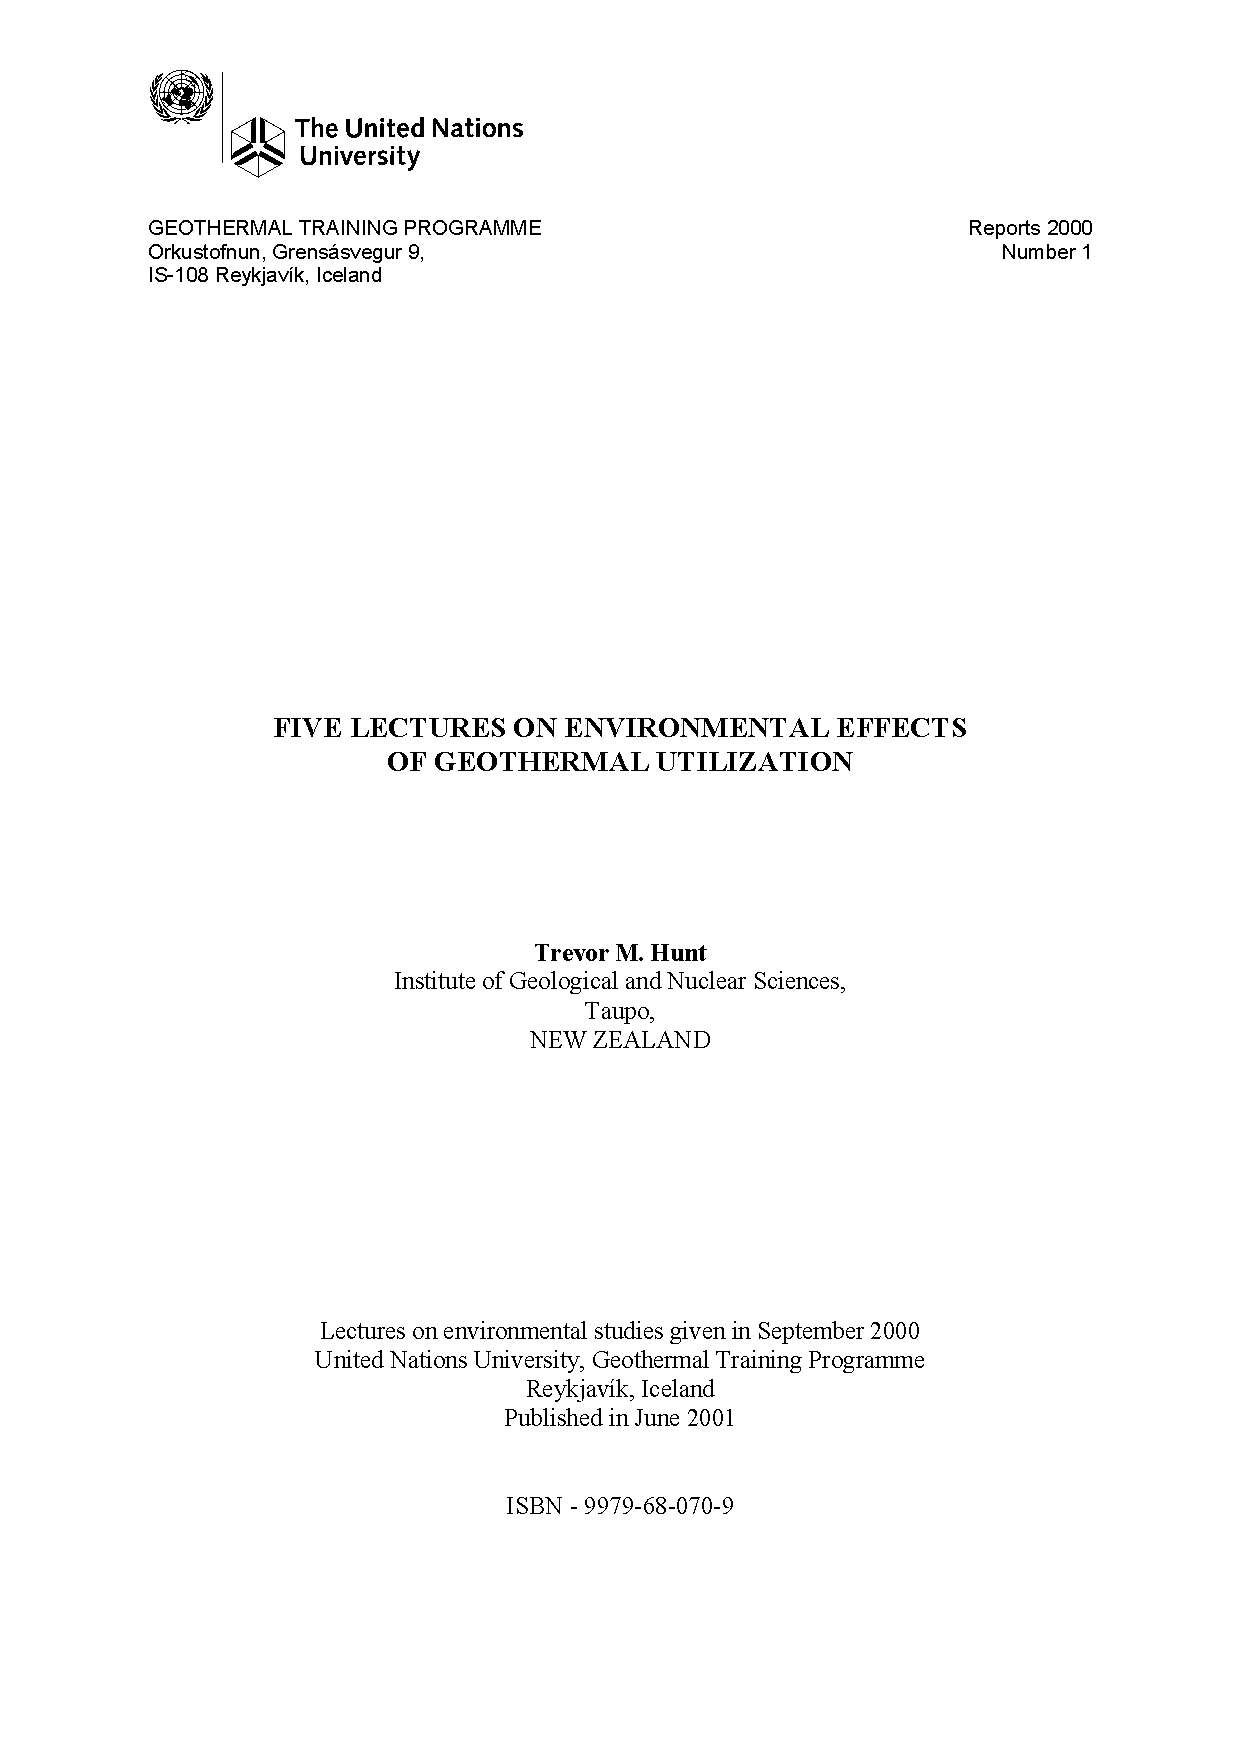
\includepdf[pages=-,fitpaper, angle=0]{./HuntSelect.pdf}
%}

\end{document}
